\documentclass{article}

\usepackage{graphicx}
\usepackage{tikz}
\usepackage{tikzsymbols}
\usetikzlibrary{calc,patterns,shapes.geometric}
\pagestyle{empty}
\usepackage[margin=0pt]{geometry}
\geometry{papersize={14in,12in}}

\def\centerarc[#1](#2)(#3:#4:#5){\draw[#1] ($(#2)+({#5*cos(#3)},{#5*sin(#3)})$) arc (#3:#4:#5);}

\begin{document}
	\begin{figure}
		\centering
		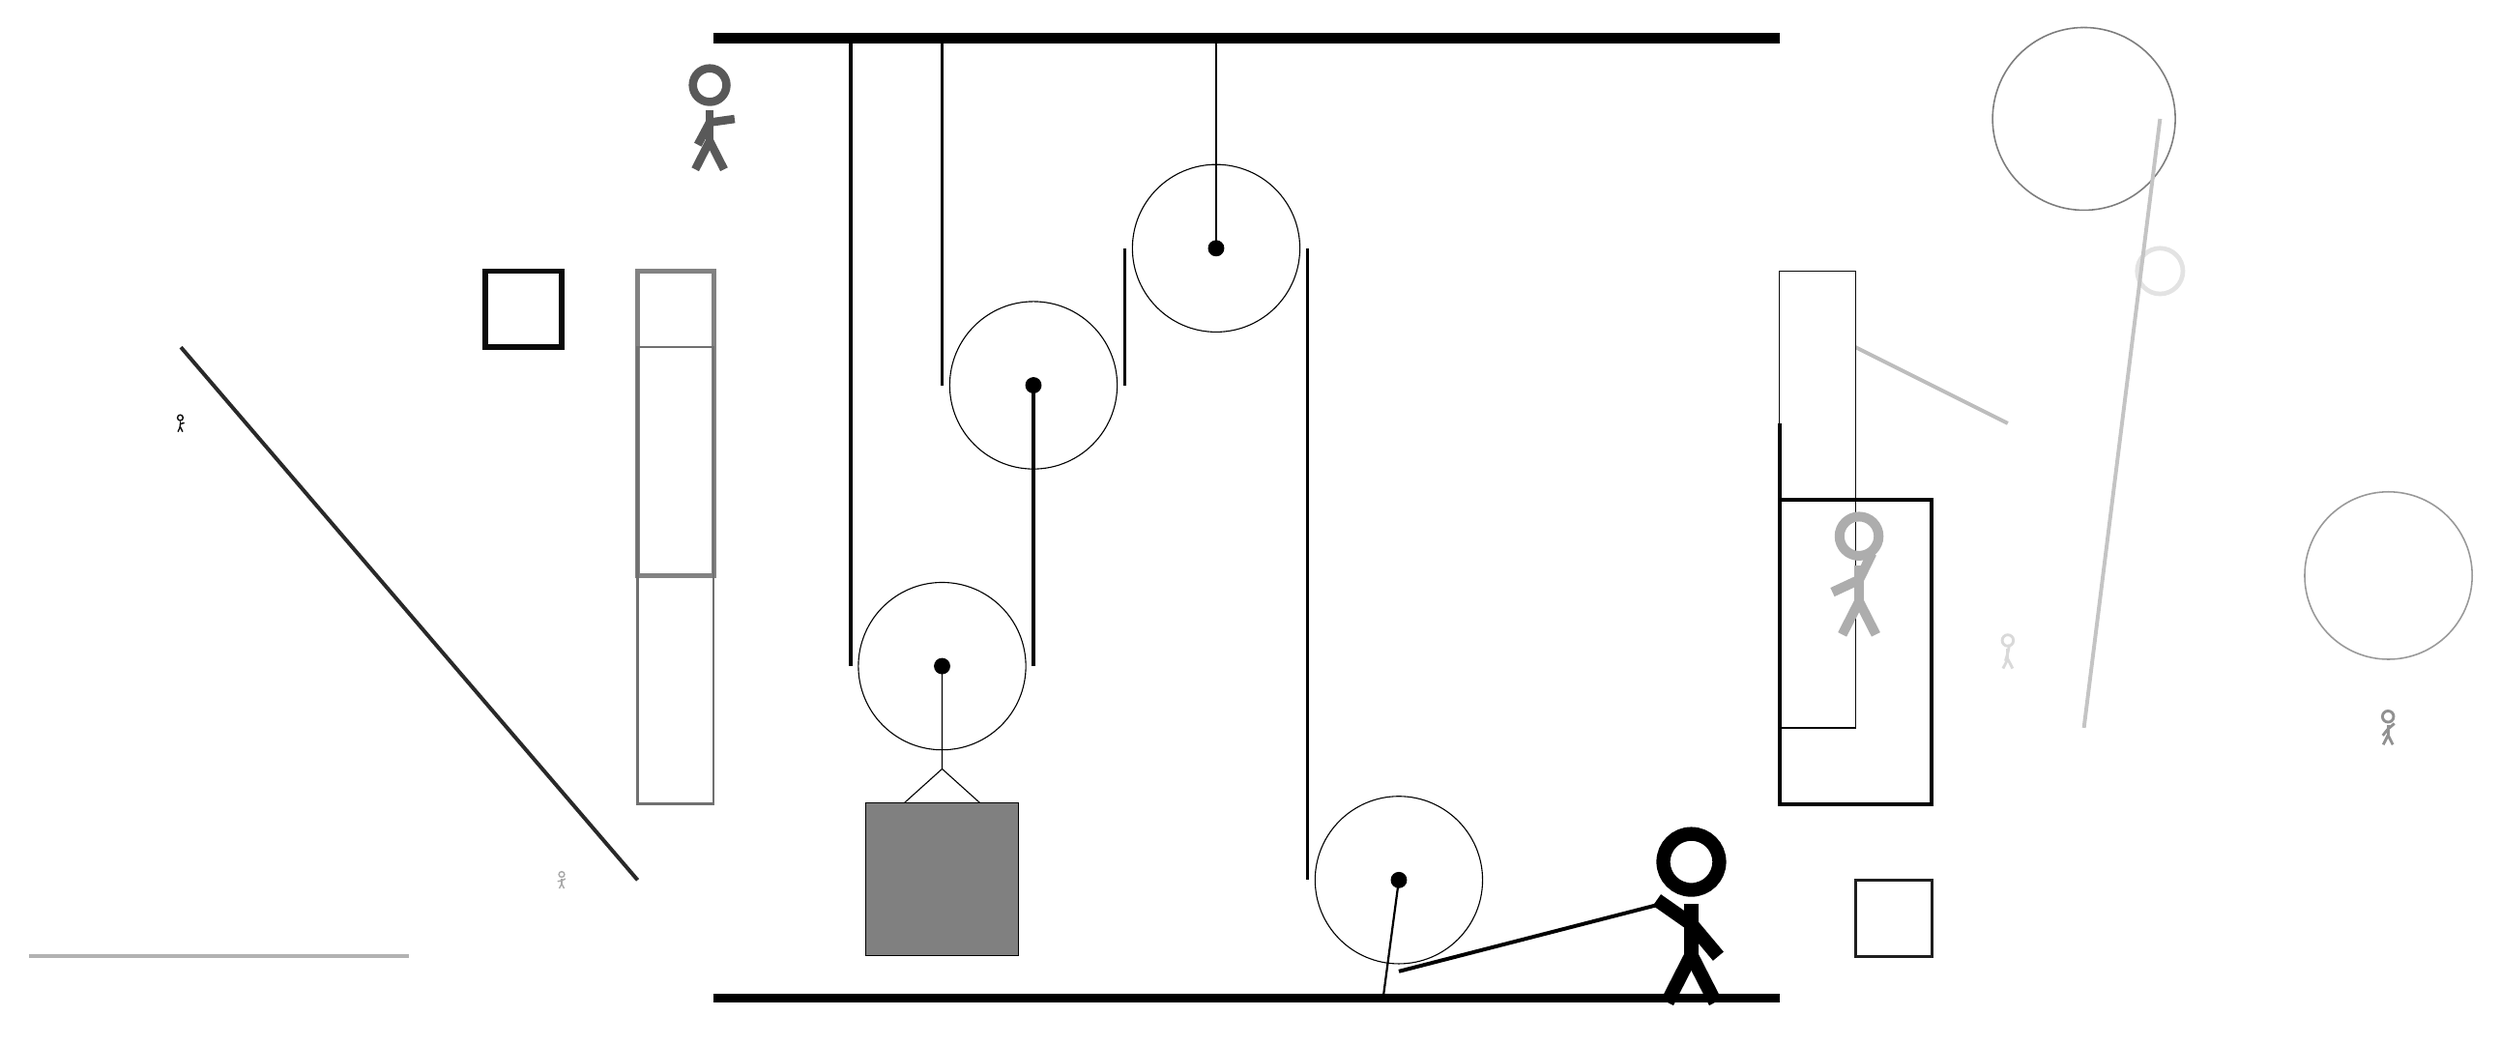
\begin{tikzpicture}
			%%%%% START %%%%%
			
			\draw[fill=black] (-2, 9) rectangle (12, 9.125);
			
			\draw (1, 0.81) circle (1.1);
			\draw[fill=black] (1, 0.81) circle (0.1);
			
			\draw (2.2, 4.5) circle (1.1);
			\draw[fill=black] (2.2, 4.5) circle (0.1);
			
			\draw (4.6, 6.3) circle (1.1);
			\draw[fill=black] (4.6, 6.3) circle (0.1);
			\draw[thick] (4.6, 6.3) -- (4.6, 9);
			
			\draw[line width=0.5mm, color=black!26](13, 5) -- (15, 4);
			
			\draw[line width=0.7mm, color=black!49] (-2, 2) rectangle (-3, 6);
			\draw[line width=0.2mm, color=black!96] (13, 6) rectangle (12, 0);
			\draw[line width=0.3mm, color=black!56] (-2, -1) rectangle (-3, 5);
			\draw[line width=0.5mm, color=black!99] (12, 3) rectangle (12, 4);
			\draw[line width=0.5mm, color=black!100] (12, 3) rectangle (14, -1);
			\draw [line width=0.6mm, color=black!11](17, 6) circle (0.3);
			
			\node[line width=0.2mm, color=black!15] at (15, 1) {\Strichmaxerl[2][74][79]};
			\draw[line width=0.5mm, color=black!84](-3, -2) -- (-9, 5);
			\node[line width=0.5mm, color=black!95] at (-9, 4) {\Strichmaxerl[1][85][15]};
			\draw [line width=0.2mm, color=black!51](16, 8) circle (1.2);
			\draw [line width=0.2mm, color=black!40](20, 2) circle (1.1);
			\draw[line width=0.5mm, color=black!30](-6, -3) -- (-11, -3);
			
			\node[line width=0.6mm, color=black!34] at (-4, -2) {\Strichmaxerl[1][11][26]};
			\node[line width=0.7mm, color=black!32] at (13, 2) {\Strichmaxerl[7][25][64]};
			\node[line width=0.2mm, color=black!43] at (20, 0) {\Strichmaxerl[2][51][41]};
			\draw[line width=0.4mm, color=black!88] (13, -2) rectangle (14, -3);
			\draw[line width=0.7mm, color=black!96] (-4, 5) rectangle (-5, 6);
			\node[line width=0.5mm, color=black!65] at (-2, 8) {\Strichmaxerl[6][62][8]};
			\draw[line width=0.5mm, color=black!23](16, 0) -- (17, 8);
			
			\draw (7.0, -2) circle (1.1);
			\draw[fill=black] (7.0, -2) circle (0.1);
			\draw[thick] (7.0, -2) -- (6.8, -3.5);
			
			\draw (1, 0.81) -- (1, -0.54) -- (0.5, -0.99) -- (1.5, -0.99) -- (1, -0.54);
			\draw[fill=black!50] (0, -0.99) rectangle (2, -2.99);
			\draw[line width=0.5mm] (-0.2, 9) -- (-0.2, 0.81);
			\centerarc[line width=0.5mm](1, 0.81)(180:360:1.2000000000000002);
			\draw[line width=0.5mm](2.2, 0.81) -- (2.2, 4.5);
			\draw[line width=0.5mm] (1.0, 9) -- (1.0, 4.5);
			\centerarc[line width=0.5mm](2.2, 4.5)(180:360:1.2000000000000002);
			\draw[line width=0.5mm](3.4, 4.5) -- (3.4, 6.3);
			\centerarc[line width=0.5mm](4.6, 6.3)(0:180:1.2000000000000002);
			\draw[line width=0.5mm] (5.8, 6.3) -- (5.8, -2);
			\centerarc[line width=0.5mm](7.0, -2)(0:90:-1.2000000000000002);
			\draw[line width=0.5mm](7.0, -3.2) -- (10.5, -2.3);
			
			\node at (10.8, -2.5) {\Strichmaxerl[10][-35][-50]};
			
			\draw[fill=black] (-2, -3.5) rectangle (12, -3.6);
			
			%%%%% END %%%%%
		\end{tikzpicture}
	\end{figure}	
\end{document}